\chapter{Adresárová štruktúra projektu}
\label{priloha-struktura}

\renewcommand{\DTcomment}[1]{\textcolor{gray}{\textit{$\triangleright$ #1}}}

Nasledujúci obrázok zobrazuje adresárovú štruktúru implementovanej aplikácie
(\texttt{lib/}).

\begin{figure}[H]
  \centering
  \begin{minipage}{0.85\textwidth}
    {\scriptsize
    \dirtree{%
      .1 project\_root/.
      .2 README.md.
      .2 docs/ \DTcomment{dokumentácia projektu, video, latex, plagát}.
      .2 lib/.
      .3 main.dart \DTcomment{vstupný bod aplikácie}.
      .3 setup.dart \DTcomment{globálne inštancie služieb}.
      .3 models/ \DTcomment{dátové modely}.
      .3 services/.
      .4 api\_service.dart \DTcomment{všetka HTTP komunikácia}.
      .4 app\_router.dart \DTcomment{definícia navigačných trás}.
      .4 session\_manager.dart \DTcomment{správa JWT a stavu prihlásenia}.
      .4 \ldots.
      .3 utils/ \DTcomment{pomocné funkcie, konštanty, témy}.
      .3 viewmodels/.
      .4 base\_consultations\_viewmodel.dart.
      .4 owner\_consultations\_viewmodel.dart.
      .4 add\_slot\_viewmodel.dart.
      .4 \ldots.
      .3 views/.
      .4 email\_input\_page.dart \DTcomment{prihlasovacia obrazovka}.
      .4 owner\_consultations\_page.dart \DTcomment{hlavná obrazovka Majiteľa}.
      .4 registration\_page.dart.
      .4 \ldots.
      .4 base\_consultations/ \DTcomment{zdieľané UI pre obe roly}.
      .4 slots/ \DTcomment{widgety pre zobrazenie slotov}.
      .4 settings/.
      .4 custom\_widgets/ \DTcomment{znovupoužiteľné widgety}.
    }}
  \end{minipage}
  \caption{Adresárová štruktúra projektu.}
  \label{fig:struktura}
\end{figure}

\chapter{Prezentačný plagát}
\label{priloha-plagat}
\begin{figure}[H]
    \centering
    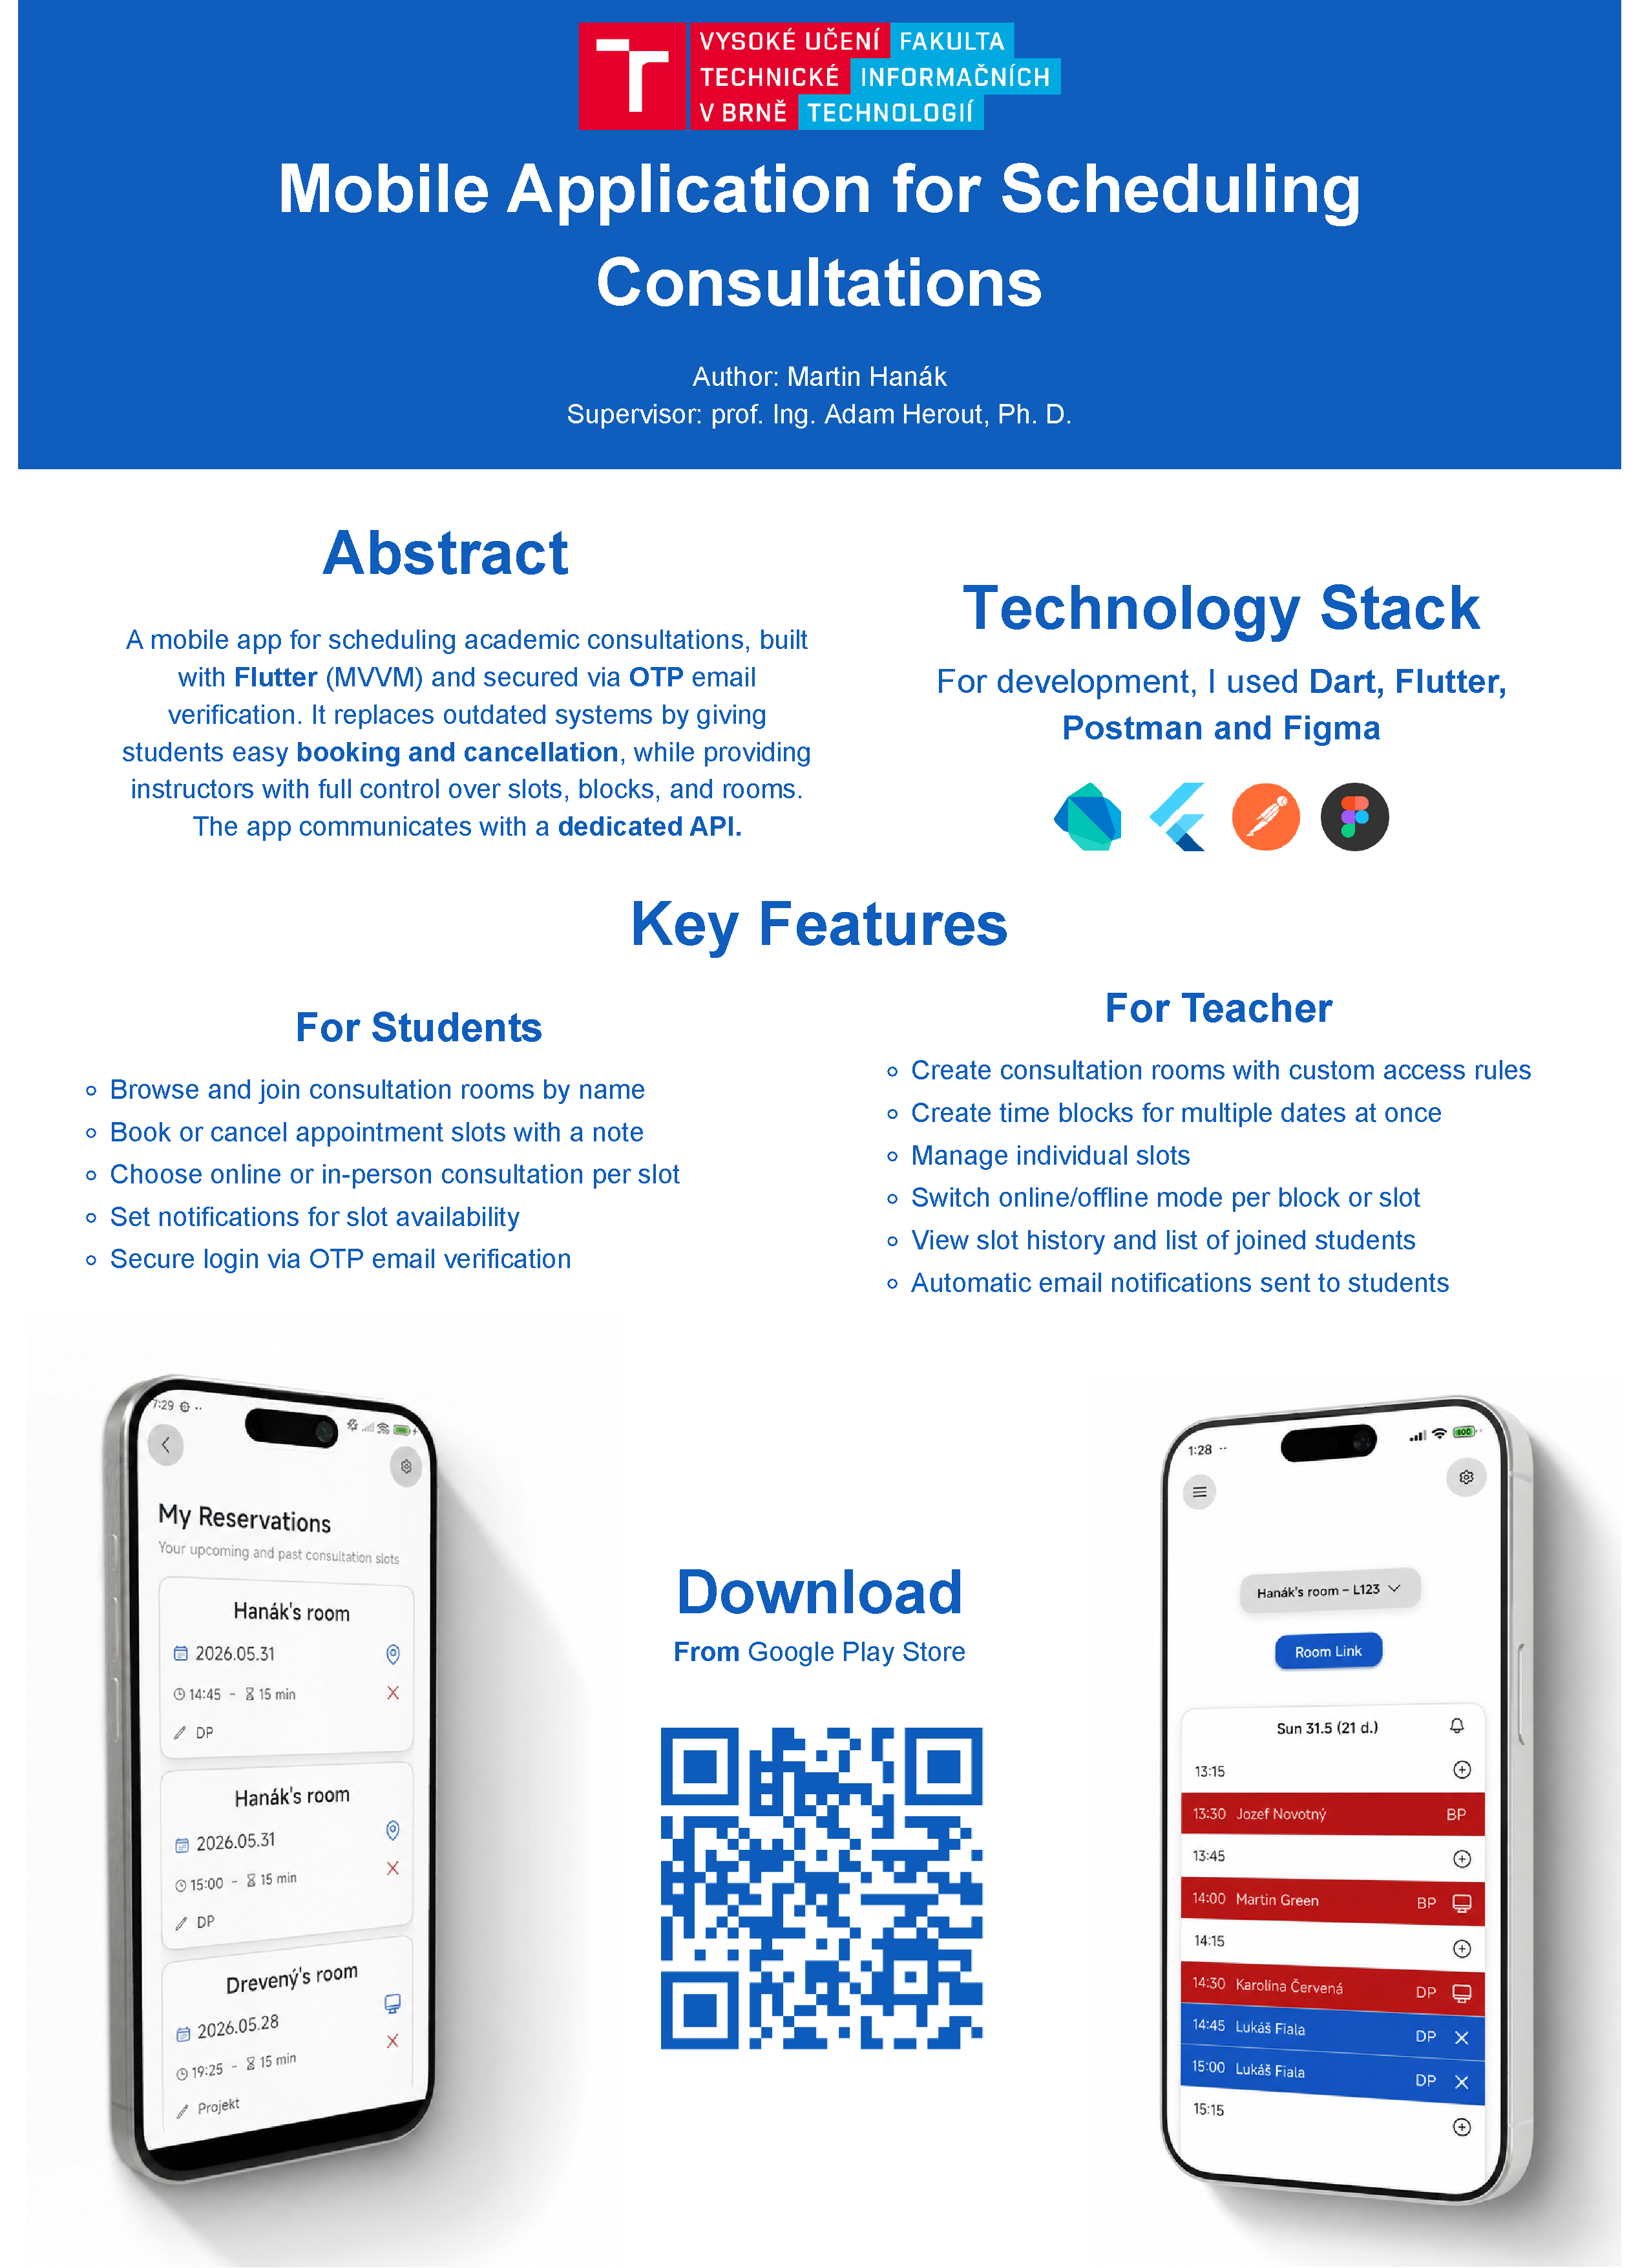
\includegraphics[width=0.7\textwidth]{obrazky-figures/office-hours-poster.pdf}
    \caption{Plagát prezentujúci mobilnú aplikáciu pre správu konzultácií, vytvorený ako súčasť obhajoby bakalárskej práce.}
    \label{fig:poster}
\end{figure}